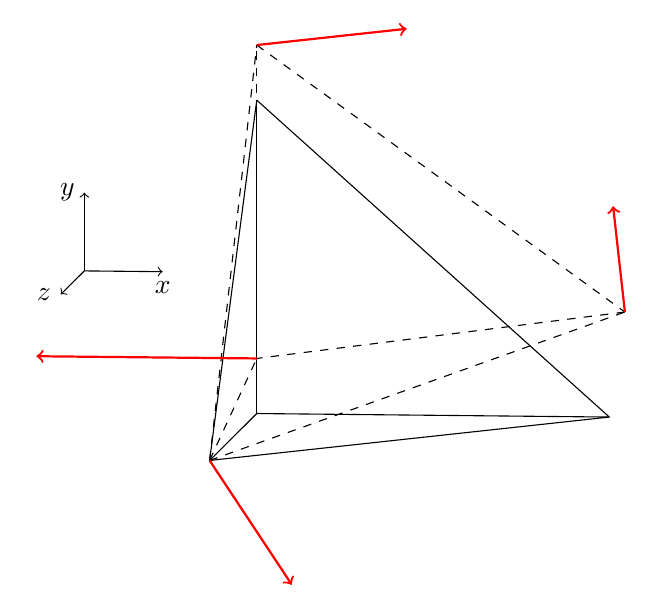
\begin{tikzpicture}
\draw[->] (-0.980017,2.03987) -- (0.0149875,2.0299);
\node[below] at (0.0149875,2.0299) {$x$};
\draw[->] (-0.980017,2.03987) -- (-0.980017,3.03487);
\node[left] at (-0.980017,3.03487) {$y$};
\draw[->] (-0.980017,2.03987) -- (-1.27952,1.74186);
\node[left] at (-1.27952,1.74186) {$z$};
\draw (1.20966,0.228594) -- (1.20966,4.20861);
\draw (1.20966,4.20861) -- (5.68718,0.183744);
\draw (5.68718,0.183744) -- (1.20966,0.228594);
\draw (0.610658,-0.367414) -- (1.20966,0.228594);
\draw (0.610658,-0.367414) -- (1.20966,4.20861);
\draw (0.610658,-0.367414) -- (5.68718,0.183744);
\draw[dashed] (1.20966,0.928164) -- (1.20966,4.90818);
\draw[dashed] (1.20966,4.90818) -- (5.88499,1.51754);
\draw[dashed] (5.88499,1.51754) -- (1.20966,0.928164);
\draw[dashed] (0.610658,-0.367414) -- (1.20966,0.928164);
\draw[dashed] (0.610658,-0.367414) -- (1.20966,4.90818);
\draw[dashed] (0.610658,-0.367414) -- (5.88499,1.51754);
\draw[->,thick,red] (5.88499,1.51754) -- (5.73524,2.86104);
\draw[->,thick,red] (1.20966,0.928164) -- (-1.58879,0.956196);
\draw[->,thick,red] (1.20966,4.90818) -- (3.11335,5.11487);
\draw[->,thick,red] (0.610658,-0.367414) -- (1.65516,-1.94563);
\end{tikzpicture}